\section{Regularised observables and reflection positivity}\label{cl:app:flow}

Gradient flow offers smooth gauge-covariant observables at positive flow
time. Its perturbative renormalisation theorem \cite{LW11} assumes that
the underlying four-dimensional theory has been renormalised; it does
not supply the nonperturbative correlation estimates in
Section~\ref{cl:sec:retention}. A second issue is that temporal smoothing
can destroy reflection positivity. We give a direct counterexample and
then a support-preserving construction that avoids this particular
obstruction. Spatial flow has also been used to avoid temporal smearing
in lattice spectral measurements \cite{SS23}.

\subsection{Reflection commutation is insufficient}
Let $\omega>0$ and $s>0$. Heat smoothing of the one-dimensional free
massive covariance gives the stationary Gaussian covariance
\[
C_s(t)=\int_{\R}e^{ipt}
       \frac{e^{-2s(p^2+\omega^2)}}{p^2+\omega^2}\,\frac{dp}{2\pi}.
\]
This is a positive covariance: its Fourier density is nonnegative.
The smoothing commutes with reflection $t\mapsto-t$.
All its derivatives exist by Gaussian decay. Put
\[
A=-C_s''(0)=\int_{\R}\frac{p^2e^{-2s(p^2+\omega^2)}}{p^2+\omega^2}
                  \,\frac{dp}{2\pi}>0,
\quad
B=\int_{\R}\frac{p^4e^{-2s(p^2+\omega^2)}}{p^2+\omega^2}
                  \,\frac{dp}{2\pi}>0.
\]
\begin{proposition}\label{cl:prop:flow-rp-fails}
The Gaussian law with covariance $C_s$ is not reflection positive for
any $s>0$, even for bounded smooth-cylinder positive-time tests.
\end{proposition}
\begin{proof}
For a positive-time linear test $F_h=X(h)-X(2h)$, its reflected
quadratic form is
\[
q(F_h)=C_s(2h)-2C_s(3h)+C_s(4h).
\]
Taylor's theorem, evenness and $|C_s^{(4)}(t)|\le B$ give
\[
q(F_h)\le-Ah^2+\frac{2^4+2\cdot3^4+4^4}{24}Bh^4
=-Ah^2+\frac{217}{12}Bh^4.
\]
Choose $0<h^2\le6A/(217B)$. Then $q(F_h)\le-Ah^2/2<0$.
Point evaluations may be replaced by unit-integral smooth smears in
small neighbourhoods of $h$ and $2h$, both contained in $(0,\infty)$.
Continuity of $C_s$ preserves the strict negative sign for sufficiently
small neighbourhoods. Finally choose smooth bounded truncations
$\varphi_M$ of the identity with $|\varphi_M(x)|\le|x|$ and
$\varphi_M(x)\to x$. The truncated tests converge in Gaussian $L^2$.
Reflection is an $L^2$ isometry, so Cauchy--Schwarz implies convergence
of their reflected quadratic forms. These remain negative for large $M$.
\end{proof}

The example concerns a free Gaussian covariance, not an interacting
Wilson measure. It disproves the general inference from reflection
commutation to reflection positivity for temporally smoothed observables.

\subsection{A construction preserving the positive-time algebra}
Let $(\Omega,\mu)$ carry a measure-preserving involution $\vartheta$ and
a positive-time algebra $\mathcal A_+$ on which
$q_\mu(F)=\int\overline{F\circ\vartheta}F\,d\mu\ge0$.

\begin{proposition}[support-preserving regularisation]\label{cl:prop:flow-rp}
Suppose a measurable map $W$ commutes with $\vartheta$ and
$F\circ W\in\mathcal A_+$ for every $F\in\mathcal A_+$.
Then $W_*\mu$ is reflection positive on $\mathcal A_+$.
\end{proposition}
\begin{proof}
The two hypotheses give
\[
q_{W_*\mu}(F)
=\int\overline{(F\circ W)\circ\vartheta}(F\circ W)\,d\mu\ge0.
\]
\end{proof}

On a finite lattice, evolve the spatial links of each Euclidean time
slice by the negative gradient of its spatial Wilson action, leaving
temporal links unchanged. The vector field is smooth on a compact
product of groups, so its ODE has a unique solution for all finite flow
times. The flow on one slice depends only on that slice. Uniqueness
and reflection symmetry make the flow commute with time reflection.
It therefore meets both hypotheses of
Proposition~\ref{cl:prop:flow-rp}, for the algebra generated by spatial
links on positive-time slices. Gauge covariance follows because the
action and product bi-invariant metric are gauge invariant.

\begin{figure}[htbp]
\centering
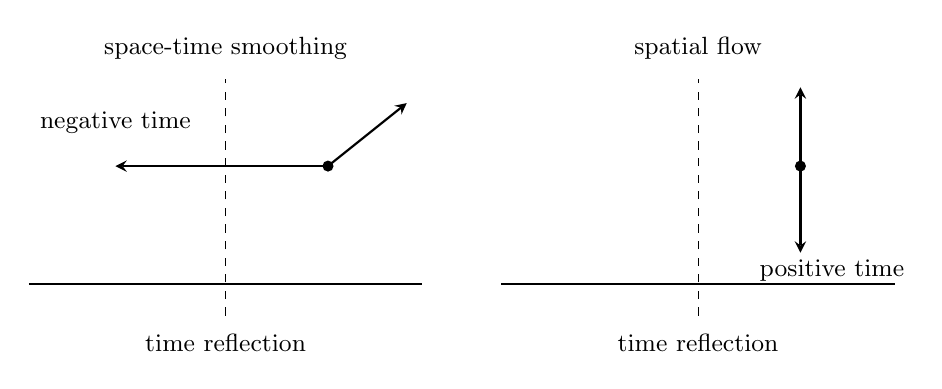
\begin{tikzpicture}[x=1cm,y=1cm,>=stealth,every node/.style={font=\small}]
\draw[thick] (0,0)--(5,0);\draw[thick] (6,0)--(11,0);
\draw[dashed] (2.5,-.4)--(2.5,2.6);
\draw[dashed] (8.5,-.4)--(8.5,2.6);
\node at (2.5,-.75){time reflection};\node at (8.5,-.75){time reflection};
\node at (2.5,3){space-time smoothing};\node at (8.5,3){spatial flow};
\fill (3.8,1.5) circle (2pt);\fill (9.8,1.5) circle (2pt);
\draw[->,thick] (3.8,1.5)--(1.1,1.5);
\draw[->,thick] (3.8,1.5)--(4.8,2.3);
\draw[->,thick] (9.8,1.5)--(9.8,.4);
\draw[->,thick] (9.8,1.5)--(9.8,2.5);
\node at (1.1,2.05){negative time};\node at (10.2,.17){positive time};
\end{tikzpicture}
\caption{Temporal smoothing can use fields across the reflection plane.
Spatial flow stays within each time slice and preserves the positive-time
algebra. The diagram describes support, not a continuum existence theorem.}
\label{cl:fig:flow-support}
\end{figure}

This construction proves finite-lattice reflection positivity for the
stated observables. It does not prove their continuum convergence,
rotation invariance or nonzero retained spectral mass. At fixed physical
flow time their lattice dependence is not confined to a fixed stencil.

\subsection{Quantitative approximation and large-field budgets}
If $F,G\in L^2(\mu)$ and $\|F-G\|_2\le\varepsilon$, reflection
invariance and Cauchy--Schwarz give
\begin{equation}\label{cl:eq:rp-error}
|q_\mu(F)-q_\mu(G)|
\le\varepsilon(\|F\|_2+\|G\|_2)
\le\varepsilon(2\|F\|_2+\varepsilon).
\end{equation}
Indeed change one factor at a time in the reflected product. Thus an
approximation by positive-time tests preserves positivity in a limit
when its right-hand error tends to zero and the reflected correlations
converge. A small fixed error is insufficient.

For a bad event $B$, H\"older's inequality supplies the compatible
moment requirement
\[
\|F\mathbf1_B\|_2\le\|F\|_q\mu(B)^{1/2-1/q}\qquad(q>2).
\]
For example, suppose $|F_a|\le Ca^{-d}$ and at most $C_Va^{-4}$
candidate blocks meet a fixed physical region. Assume each block is
bad with probability at most $C_Be^{-c\beta(a)}$, where
$\beta(a)\ge\kappa\log(1/a)-B_0$. No independence is needed for
the union bound, which gives
\[
\|F_a\mathbf1_{B_a}\|_2
\le C(C_VC_Be^{cB_0})^{1/2}
     a^{(c\kappa-4)/2-d}.
\]
It tends to zero if $c\kappa>4+2d$. This is a sufficient exponent
budget under the displayed assumptions, not a proved Wilson tail bound.
Centering the difference only decreases its $L^2$ norm. To use
\eqref{cl:eq:rp-error} with a positive-time truncation, the event
$B_a$ must itself be measurable in the positive-time algebra; a global
bad event crossing the reflection plane need not meet that condition.
